 \documentclass[conference]{IEEEtran}

\usepackage{url}
\usepackage{hyperref}
\usepackage{amssymb,amsmath}
\usepackage{tikz}
\usetikzlibrary{calc,positioning,shapes,shadows,arrows,backgrounds,fit}

\usepackage{xspace}

\newcommand{\todo}[1]{{$\langle\!\langle$\marginpar{$\blacksquare$}\textsf{#1}$\rangle\!\rangle$}}

\definecolor{midgrey}{rgb}{0.5,0.5,0.5}
\definecolor{darkred}{rgb}{0.7,0.1,0.1}
\newcommand{\nnote}[1]{$[$\textcolor{darkred}{norbert}:~~\emph{\textcolor{midgrey}{#1}}$]$\marginpar{$\blacksquare$}}
\newcommand{\anote}[1]{$[$\textcolor{darkred}{ahmed}:~~\emph{\textcolor{midgrey}{#1}}$]$\marginpar{$\blacksquare$}}
\newcommand{\dnote}[1]{$[$\textcolor{darkred}{davide}:~~\emph{\textcolor{midgrey}{#1}}$]$\marginpar{$\blacksquare$}}

\def\CC{{C\nolinebreak[4]\hspace{-.05em}\raisebox{.4ex}{\tiny\bf ++}}}

%Davide>
\newcommand{\ls}{\{}
\newcommand{\rs}{\}}
\renewcommand{\langle}{\{}
\renewcommand{\rangle}{\}}

\newcommand{\1}{x_1}
\newcommand{\2}{x_2}
\newcommand{\3}{x_3}
\newcommand{\4}{x_4}
\newcommand{\5}{x_5}
\newcommand{\6}{x_6}
\newcommand{\7}{x_7}
\newcommand{\8}{x_8}
\newcommand{\9}{x_9}

\newcommand{\pcasso}{\textsc{Pcasso}\xspace}
\newcommand{\coprocessor}{\textsc{Coprocessor}\xspace}
\newcommand{\riss}{\textsc{Riss}\xspace}
\newcommand{\cubeandconquer}{\textsc{CubeAndConquer}\xspace}
\newcommand{\splitter}{\textsc{Splitter}\xspace}
\newcommand{\penelope}{\textsc{PeneLoPe}\xspace}
\newcommand{\manysat}{\textsc{ManySAT}\xspace}
\newcommand{\satelite}{\textsc{SatELite}\xspace}
\newcommand{\minisat}{\textsc{Minisat 2.2}\xspace}
\newcommand{\glucose}{\textsc{Glucose 2.2}\xspace}
\newcommand{\ppfolio}{\textsc{Ppfolio}\xspace}
\newcommand{\pfoliouzk}{\textsc{PfolioUZK}\xspace}
\newcommand{\plingeling}{\textsc{Plingeling}\xspace} %Thy shall never try to spell this
\newcommand{\lingeling}{\textsc{Lingeling}\xspace}

\newcommand{\T}{\mathcal{T}}
\newcommand{\A}{\mathcal{A}}


\newcommand{\tuple}[1]{{\langle{#1}\rangle}}
\newcommand{\setdef}[2]{{\left\{#1\,\mid \,#2\right\}}}

\newcommand{\F}{F}
\newcommand{\Fa}{G}
\newcommand{\J}{J}

\def\ngt#1{\overline{#1}}
\newcommand{\Dec}[1]{\dot{#1}}

\newcommand{\mfalse}{\bot}
\newcommand{\mtrue}{\top}
\def\NP{\mathcal{NP}}


\newcommand{\Lits}{\mathsf{lits}}
\newcommand{\Atoms}{\mathsf{vars}}
\newcommand{\Reduct}[2]{{#1|}_{{#2}}}
\newcommand{\EmptyClause}{[\,]}

\newcommand{\DecideR}{\rightsquigarrow_{dec}}
\newcommand{\UnitR}{\rightsquigarrow_{unit}}
\newcommand{\LearnR}{\rightsquigarrow_{learn}}
\newcommand{\BackR}{\rightsquigarrow_{back}}

\newcommand{\SAT}{\textit{SAT}\xspace}
\newcommand{\UNSAT}{\textit{UNSAT}\xspace}

%
\newcommand{\with}{::}

\newcommand{\tableRowBreak}{\\}
\newcommand{\tableColSpace}{@{\hspace{1.5em}}}
\newcommand{\tableColSmallSpace}{@{\hspace{1ex}}}
\newcommand{\tableVSpace}{-2ex}
\newcommand{\figureVSpace}{-2ex}
\newcommand{\proofspace}{-1ex}
\newcommand{\definitionspace}{-0.5ex}




% Number Sets
\newcommand{\Naturals}{\mathbb{N}}
\newcommand{\Ints}{\mathbb{Z}}
\newcommand{\Reals}{\mathbb{R}}

\newcommand{\Program}[1]{\textsc{#1}}
\newcommand{\Rewrite}{\leadsto}

\newcommand{\ShareR}{\Rewrite_{\mathsf{share}}}
\newcommand{\AddR}{\Rewrite_{\mathsf{add}}}
\newcommand{\DelR}{\Rewrite_{\mathsf{del}}}
\newcommand{\SatR}{\Rewrite_{\mathsf{sat}}}
\newcommand{\UnsatR}{\Rewrite_{\mathsf{unsat}}}
\newcommand{\CMR}{\Rewrite_{\mathsf{\equiv}}} % Clause Management Rule
\newcommand{\InprocessR}{\Rewrite_{\mathsf{inp}}} % Clause Management Rule
\newcommand{\RestrictedInprocessR}{\Rewrite_{\mathsf{rinp}}} % Clause Management Rule

\newcommand{\Domain}{\mathsf{dom}}
%\newcommand{\Reduct}[2]{{#1|}_{{#2}}}
%\newcommand{\EmptyClause}{[\,]}

\newcommand{\Neg}[1]{\overline{#1}}

%\newcommand{\SAT}{\mathsf{SAT}\xspace}
%\newcommand{\UNSAT}{\mathsf{UNSAT}\xspace}



\begin{document}
	
% paper title
\title{\textsc{Pcasso} -- a Parallel CooperAtive Sat SOlver}

% author names and affiliations
% use a multiple column layout for up to three different
% affiliations
\author{
 \IEEEauthorblockN{Davide Lanti}
 \IEEEauthorblockA{Free University of Bolzano\\Italy}
 \and
 \IEEEauthorblockN{Ahmed Irfan}
 \IEEEauthorblockA{ Fondazione Bruno Kessler, Italy\\
 University of Trento, Italy}
 \and
\IEEEauthorblockN{Norbert Manthey}
\IEEEauthorblockA{TU Dresden\\Germany}
}

% conference papers do not typically use \thanks and this command
% is locked out in conference mode. If really needed, such as for
% the acknowledgment of grants, issue a \IEEEoverridecommandlockouts
% after \documentclass

% use for special paper notices
%\IEEEspecialpapernotice{(Invited Paper)}

\maketitle

% the abstract is optional
\begin{abstract}
The SAT solver \pcasso is a parallel SAT solver based on partitioning the search space iteratively and using clause sharing among the nodes.
\end{abstract}

\section{Introduction}

The major difference to last years version of \pcasso is the update of the formula simplifier \coprocessor. 
The remaining configuration of the tool remained the same. 
We only adapted the internal data structures to the structures of \riss to match this years version 4.27~\cite{riss427}. 

%Picture and all that!
\pcasso proceeds by creating and solving partitions of the input instance.
Partitions are created through \emph{partition functions}, where a partition function is a function $\phi$ such that, given a  formula $F$ and a natural number $n \in \mathbb{N^+}$, ${\phi(F,n) := (F_1, \ldots, F_n)}$, where ${F \equiv F_1 \lor \ldots \lor F_n}$ and each pair of partitions is disjoint: ${i \neq j \in [1,n]}$, ${F_i \land F_j \models \bot}$. 
Without loss of generality we assume that partitions $F_1, \ldots, F_n$ are always of the form ${F \land K_1, \ldots, F \land K_n}$, where $K_1, \ldots, K_n$ are sets of clauses, called \emph{partitioning constraints}.
By iteratively applying the partition function to a formula $F$, a \emph{partition tree} 
%like the one in \emph{Figure}~\ref{f:iterative-partitioning} 
is produced. 
Nodes in the partition tree are tagged with their \emph{positions}: the root node $F$ is tagged with the empty position $\epsilon$; the i-th successor (from left to right) of a node $F^p$ at position $p$ is the node $F^{pi}$ (see Figure~\ref{fig:position-based}).
Please notice that, as positions are strings, the standard \emph{prefix} relation among strings ($<$) is defined for positions as well.

% This instructions provide general guidelines on what a good solver description contains. 
% The sectioning may be changes, as long as the required details are presented.
% 
% Notice that the solver description should be specific to the particular version of your solver that 
% is submitted to SAT Competition 2013. Even if you have previously published a paper
% on a previous version of your solver, simply providing such an earlier paper 
% or just referring to such a paper does not meet the requirements for solver descriptions
% for SAT Competition 2013.
% 
% Notice also that, following the principles of scientific writing, necessary references
% to known techniques implemented in your solver should be provided.
% Example reference: \cite{JeroslowWang:1990}
% 
% Naming convention for the solver description PDF: 
% name the file according to the name of your solver.
% 
% Make sure that page numbering is turned off.

\section{Main Techniques}

% Which algorithmic paradigm(s) the solver is based on: CDCL, SLS, look-ahead, hybrid (of what), portfolio (of what type of solvers, which solvers) ? 
% 
% What further solving techniques are used (e.g. preprocessing, restart/learning/... strategies, ...)?

%Partition based on look-ahead, solving with glucose. information sharing.
The partition function used in \pcasso is \emph{tabu scattering}, which is an extension of \emph{scattering}~\cite{HJN06}. 
The idea of scattering is to define each partitioning constraint as conjunctions of \emph{cubes} \cite{HKWB12}, where a cube is a formula ${Q:=\langle C_1, \ldots, C_n\rangle}$ such that $|C_i| = 1$, for each $1 \le i \le n$. 
Observe that the negation of a cube ${Q:=\langle \ls l_1 \rs, \ldots, \ls l_n \rs \rangle}$ is the clause $\ls \ngt{l_1}, \ldots, \ngt{l_n} \rs$. 
More precisely, given a formula $F_0$ and an integer $n$, the $n$ partitions $F_1, \ldots, F_n$ are created by using $n-1$ cubes $Q_1, \ldots, Q_{n-1}$ and applying them according to the following schema:  
${F_1 := F_0 \land Q_1}$; ${F_{m+1} := F_0 \land ( \bigwedge \limits_{i=1}^{m}{\ngt{Q_{i}}} ) \land Q_{m+1} (1 \le m < n-1)}$; 
and finally $F_n := F_{0} \land \bigwedge \limits_{i=1}^{n-1}{\ngt{Q_{i}}}$.
\emph{Tabu scattering} adds the restriction to scattering that a variable used in one cube must not be used in the cubes for creating the remaining partitions.
Using tabu scattering, we diversify the search more.
%
%Another observation is that scattering does not always create partitions that have equal difficulty in terms of solving time.
%Due to this difference, consider a scenario that the solver has some idle resources, so the solver creates partitions of some running unsolved node $(F^p,?,\blacktriangleright)$ in the partition tree, but it may happen that $(F^p,?,\blacktriangleright)$ is very close to find the result~$\bot$ and thus the solver may waste resources on the newly created partitions. We propose a solution to decrease the chance of this scenario to happen, by sorting the child nodes in decreasing order of difficulty level; this way the solver will create partitions of more difficult node first than the less difficult nodes, avoiding the above scenario.
%We predict the difficulty level of a node by a simple heuristic that counts the number of propagated literals: the higher the number of propagated literals, the lower the estimated difficulty of the analyzed formula.
%
\pcasso uses lookahead techniques~\cite{HvM09HBSAT} for choosing the literals (in cubes). 
%In particular it chooses variables with the maximum \emph{mixdiff} score~\cite{HvM09HBSAT}. 
%The score \emph{mixdiff} of a variable is the product of the \emph{diff} score of each polarity of the variable.
%We calculate the \emph{diff} score of the polarity of a variable by applying lookahead, and use the following weighted sum: 
%$0.3$ times the number of propagated literals plus $0.7$ times the number of newly created binary clauses.
%After choosing the variable with the maximum \emph{mixdiff} score, we choose the polarity of the variable that has the lowest \emph{diff} score for creating cubes. 
We also use the following reasoning techniques: failed literals, necessary assignments, pure literals, and add learned clauses to the partition constraints. 
Techniques like constraint resolvent, double lookahead, and adaptive pre-selection heuristics are also used as proposed in the literature~\cite{HvM09HBSAT}. 
%It is the first time that lookahead and scattering is combined for creating partitions.
%Previously lookahead has already been used in \cubeandconquer for creating partitions, but without scattering~\cite{HKWB12,THB12}. 

%Hyv\"arinen~\cite{HJN10} identifies two strategies for solving nodes in the partition tree: \emph{plain partitioning} and \emph{iterative partitioning}. 
To describe the \emph{node-state} of a node $F^p$ at a certain point of execution we use a triple $(F^p,s,r)$ where $s \in \{\top, \bot, ?\}$ ($\top$ indicates that an incarnation found a model for the node, whereas $\bot$ indicates that an incarnation proved unsatisfiability of $F^p$; finally, $?$ indicates that the node has not been solved yet) and $r \in  \{\blacktriangleright, \blacksquare\}$ (indicating whether an incarnation is \emph{running} on $F^p$ or not, respectively). 
%
Given the notion of node-state, 
%we can easily differentiate between plain partitioning and iterative partitioning: 
\pcasso exploits the \emph{overlapped solving} strategy if two incarnations are allowed to run at the same time on nodes $F^p, F^q$ such that $p \le q$. 
%Otherwise, the solver is said to be exploiting the plain partitioning strategy. 
In order to solve an unsatisfiable node $F^p$, either $F^p$ has to be directly solved by some incarnation or each child node $F^{pi}$ has to be solved. 
%Hyv\"arinen shows in \cite{HM12} that solving each of these children can be more expensive (in terms of required time) than solving the father node directly. 
%A consequence of this fact is that overlapped solving is superior to non-overlapped solving; this claim is formally proved in~\cite{HJN10}.
%\textsc{Splitter} uses a solving time limit for each node in the partition tree, proposed in~\cite{HJN10} for grid environment.
There is no limit on the solving time for each node.
%To give the intuition about our idea, we first define the \emph{ideal solving time limit:} a solving time limit is \emph{ideal} if the given CNF formula is solved within that limit.
%Given an unsatisfiable CNF formula that we solve with overlapped solving,  
%By over-approximating the ideal limit, we overcome this problem. 
%
Per variable, VSIDS activity and progress saving are shared from parent to child nodes. 
%When \pcasso starts solving, the root node and the nodes at the partition tree level one start at almost the same time. 
%The nodes at partition tree level greater than one are usually created after some time, so we initialize their search process with the VSIDS and progress saving information of their parent, because the child node searches in the sub-search space of its parent and whatever is learned by the parent search can help the solving child node as well.

\begin{figure*}
\centering
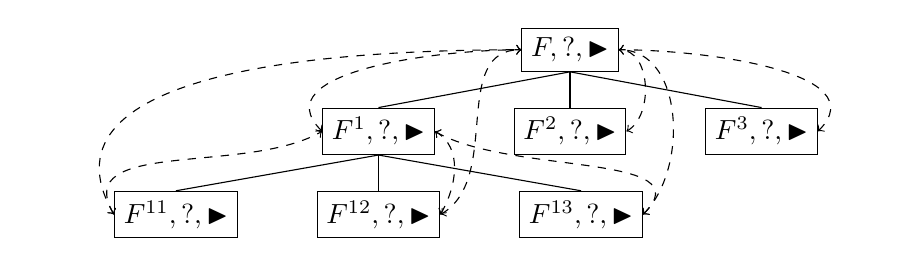
\begin{tikzpicture}
\node [rectangle, draw] (root) {$F,?,\blacktriangleright$};
\node [rectangle, draw, below=3ex of root] (p2) {$F^2,?,\blacktriangleright$};
\node [rectangle, draw, left=of p2] (p1) {$F^1,?,\blacktriangleright$};
\node [rectangle, draw, right=of p2] (p3) {$F^3,?,\blacktriangleright$};
%\node [rectangle, draw, right=0.9of p3] (p4) {$F_4,?,\blacktriangleright$};
\draw (root.south) -- (p1.north);
\draw (root.south) -- (p2.north);
\draw (root.south) -- (p3.north);
%\draw (root.south) -- (p4.north);
\node [rectangle, draw, below=3ex of p1] (p12) {$F^{12},?,\blacktriangleright$};
\node [rectangle, draw, left=of p12] (p11) {$F^{11},?,\blacktriangleright$};
\node [rectangle, draw, right=of p12] (p13) {$F^{13},?,\blacktriangleright$};
%\node [rectangle, draw, right=0.6of p13] (p14) {$F_{14},?,\blacktriangleright$};
\draw (p1.south) -- (p11.north);
\draw (p1.south) -- (p12.north);
\draw (p1.south) -- (p13.north);
%\draw (p1.south) -- (p14.north);
\draw [dashed, <->] (p11.west) to [in=180, out=120] (root.west);
\draw [dashed, <->] (p12.east) to [in=180, out=30] (root.west);
\draw [dashed, <->] (p13.east) to [in=0, out=45] (root.east);
\draw [dashed, <->] (p1.west) to [in=180, out=135] (root.west);
\draw [dashed, <->] (p2.east) to [in=0, out=30] (root.east);
\draw [dashed, <->] (p3.east) to [in=0, out=45] (root.east);
\draw [dashed, <->] (p11.west) to [in=210, out=120] (p1.west);
\draw [dashed, <->] (p12.east) to [in=330, out=60] (p1.east);
\draw [dashed, <->] (p13.east) to [in=330, out=45] (p1.east);
\end{tikzpicture}

\caption{Visualization of a partition tree with clause sharing and overlapped solving: The dashed lines represent the possible sharing with position based tagging.}
\label{fig:position-based}
\end{figure*}

Learned clauses are shared between incarnations to intensify the search.
%In the overlapped solving, we cannot share each learned clause with every incarnation, because partitioning constraints can contribute to the learning of a clause, and so the clause cannot always be a logical consequence of partition formulas solved by other incarnations. 
A learned clause is considered \emph{unsafe} if it belongs to partitioning constraints, or it is obtained by a resolution derivation involving one or more unsafe clauses. A clause that is not unsafe is called \emph{safe}. 
The main intuition here is that sharing unsafe clauses might affect the soundness of the procedure, and thus it should be forbidden. 
%Sharing in the overlapped solving has been further improved by \emph{position-based clause tagging}~\cite{davide}.
%The idea of safe and unsafe clause is extended to work per sub-partition tree: 
Concerning \pcasso, a learned clause is shared in a sub-partition tree if it is safe in that sub-partition tree.
This information can be calculated by tagging each clause with the position of the sub-tree where the clause is valid (\emph{position-based} tagging \cite{davide}).
%Most parallel solvers use a static measure for sharing clauses. \splitter shares only binary clauses~\cite{davide}. 
We propose a dynamic learned clause sharing scheme, that is based on LBD scores~\cite{AS09}.
A learned clause is eligible for sharing by an incarnation if the LBD score of this clause in the incarnation is lower than a fraction $\delta$ of the global LBD average of the incarnation.
In \pcasso, we use $\delta=0.5$.

\pcasso uses different restart policies and different clause cleaning policies for the nodes, depending whether the node is root, leaf or middle (not root and not leaf). 

%During our experiments we have observed, on some instances, that the height of the partition tree grows until it hits the number of parallel resources. 
%This means that there is only one unsolved node at each partition level of the partition tree.
\pcasso can have a scenario where there is only one unsolved node at some partition level.
We call this scenario the \emph{only child scenario}. 
%
%\begin{figure}[t]
%  \centering
%\input{tikz-image/play-stop-tikz.tex}
%\caption{The given snapshot shows the only child scenario for four computation units: for each node, only a single child is still unsolved, and all other nodes are evaluated to $\bot$.}
%\label{fig:only-child}
%\end{figure}
%
%\begin{example}
%Figure~\ref{fig:only-child} shows an extreme case of only child scenario for a solver with four available resources.
%You can see that only one node is unsolved at each level of the partition tree, i.e. the nodes solving the partitions $F$, $F^2$, $F^{21}$, $F^{213}$ are unsolved and running.
%\end{example} 
%
Consider that if the only child scenario happens at some level of the partition tree, then there are two cases:
%\begin{itemize}
%\item 
i) the parent node is looking into the search space which has been solved by one of its children already,
%\item 
ii) the parent node is looking into the same search space where its unsolved children are looking.
%\end{itemize}
In either case, we have the risk of doing redundant work.
We propose an approach to get out of this scenario by reintroducing the solving limit in a node that has only one unsolved child (\textsc{Avoid}).
%, as we can say with a high probability that the partitioning function is not void (as all the partitions are solved except one).
To be on safe side, we do not apply this limit for the root node. %, so that we are not slower than the sequential solver.
The introduced limit grows with the level of the node (level $*$ 4096 conflicts). 
Since in the only child scenario all learned clauses can be shared among the two participating nodes, we can also \textsc{Exploit} this situation, by enabling this sharing. 
In the extreme case, this configuration is very similar to portfolio solvers, where all clauses can be shared without restrictions. 
%
When clauses are tagged by position-based tagging~\cite{davide}, additional information can be obtained by performing a conflict analysis on solved unsatisfiable nodes. Consider a node $(F^p, \bot, \blacksquare)$, and let $\langle \rangle^q$ be the empty clause derived by the incarnation that solved $F^p$. Then, from the main theorem in \cite{davide}, we conclude that $\langle \rangle^q$ is the semantic consequence of the node of position $q$ in the partition tree. Observe that $q$ is a prefix $p$: $q \le p$. Consequently, not only the node at position $p$ can be marked as unsatisfiable, but also the node $F^q$ as well as all its child nodes. As a result, more incarnations can be terminated and start solving different partitions. 
We call this kind of technique \emph{conflict driven node killing}. 
A similar approach is reported in~\cite{HJN11}.
% with \emph{assumption-based} clause tagging, but the author did not report benefits from exploiting this technique. 
%Instead, our tests show an improved performance in terms of the number of solved instances. 
%However, similarly to~\cite{HJN11}, we observe an increase of the median time. 
%A reason for might be the fact that by stopping a node we prevent it from producing more shared clauses for its and above levels. 

\section{Main Parameters}

The major parameters of the solver specify the number of threads that should be used, the number of partitions that should be created for each node, and how sharing should be performed. 
For the competition, we use 12 threads, and produce 8 partitions. Furthermore, we share learned clauses according to their LBD value. 
Finally, the treatment of the only-child scenario can be specified as well. 

%For each of these parts of the solver, many parameters are provided in order to control the special behavior of the system. 
%\dnote{Big, small??? Ugly}
There are only minor magic constants that control the run time of the look-ahead procedures that are applied during partitioning, whose values have been chosen according to the literature~\cite{HvM09HBSAT}. 


\section{Special Algorithms, Data Structures, and Other Features}

% Implementation-level details: special data structures, algorithmic details, \ldots
Each node in the partition tree is associated to a \emph{pool of shared clauses}, where a pool is implemented as a vector of clauses. 
This permits to decouple the life of a shared clause from the life of the incarnation where the shared clause has been learned. 
Instead of tagging each clause with a position, clauses are tagged with integers representing a \emph{level} in the partition tree 
(root node has level zero). Observe that this is sufficient to simulate the position based approach ---that is, each incarnation working over a node $F^p$ can only access the pools placed at nodes of positions $q \le p$. 
Concurrent access to pools is regulated by standard \verb|POSIX| Read-Write locks. 

\textsc{Coprocessor} is used as preprocessor~\cite{Manthey:2012:CFC:2352219.2352264}. 


\section{Implementation details}

\pcasso is built on top of a simplified version of \riss without inprocessing and without the modifications to the CDCL algorithm, so that the implementation of clause sharing remains as simple as possible. 
The formula simplifier \textsc{Coprocessor} is used as an external tool before \pcasso is executed. 
 
% \section{SAT Competition 2014 Specifics}
% 
% \pcasso has been submitted to both the application and the crafted parallel track. 

\section{Availability}

The source code of \pcasso and \coprocessor is available for research at \url{tools.computational-logic.org}. 


% \section*{Acknowledgment}
% The authors would like to thank...

% \bigskip
% What should not be in the system description:
% \begin{enumerate}
%   \item Basic definitions related to SAT. (However, any formal notations used in the description should be defined.)
%   \item Empirical results on the solver's performance.
% \end{enumerate}

\bibliography{pcasso}
\bibliographystyle{IEEEtran}
% \bibliography{sc2013}

\end{document}


